\chapter{ Hinweise}
\label{sec:Hinweise}
\section{Allgemeine Hinweise}
\label{sec:AllgemeineHinweise}
Dies ist ein Beispiel für eine Aufzählung. Um den Abstand zwischen Aufzählung und Text sichtbar zu machen, verläuft dieser Text über zwei Zeilen
\begin{itemize}
	\item Strukturiertes Vorgehen bei der Problemlösung
	\item Kein Text zwischen Haupt- und Zwischenüberschrift
	\item Betrag und Einheit mit Leerzeichen, zum Beispiel 1 mm
	\item Zahlen bis Zehn und Einheiten ausschreiben
	\begin{itemize}
		\item im ersten Abschnitt oder im Abschnitt 1 nicht im 1. Abschnitt
		\item In einer Entfernung von einem Kilometer oder In einer Entfernung von L = 1 km, nicht In 1 km Entfernung 
		\item zehn Prozent Gewinn statt 10 \% Gewinn
		\end{itemize}
	\item Abkürzungen möglichst vermeiden, besser ausschreiben
	\begin{itemize}
	\item Zum Beispiel statt z.B.
\end{itemize}
\end{itemize}	
Dies ist der Text nach der Aufzählung. Auch hier kann man den Abstand zwischen Aufzählung und darauffolgenden Text sehen.
\clearpage
\section{Bilder untereinander und nebeneinander}
\label{sec:BilderUntereinander}
\subsection{Eine Bildunterschrift}
\label{sec:EineBildunterschrift}

\begin{figure}[ht]
  \centering
  \subfigure{
    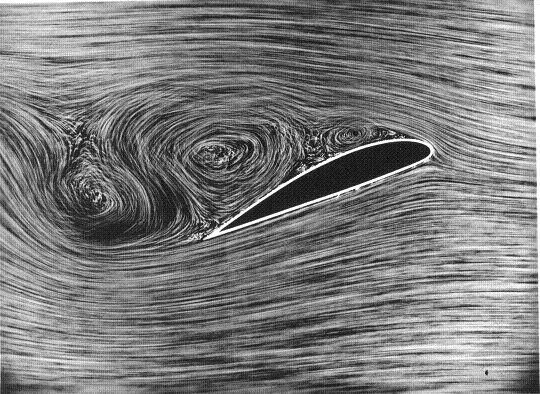
\includegraphics[width=0.5\textwidth]{stroemung1.PNG}  
  }
  \subfigure{
    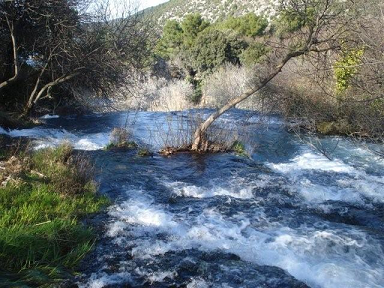
\includegraphics[width=0.35\textwidth]{stroemung2.PNG}  
  }
  \subfigure{
    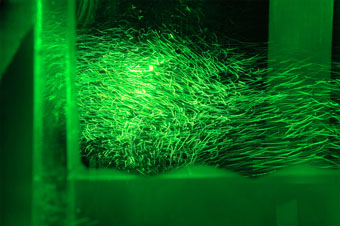
\includegraphics[width=0.25\textwidth]{stroemung3.PNG}  
  }
  \caption{Bildunterschrift}
  \label{fig:xyz1}
\end{figure} 
\clearpage

\begin{landscape}
\section{Querformat}
\label{sec:Querformat}
\begin{figure}[ht]
  \centering
  \subfigure{
    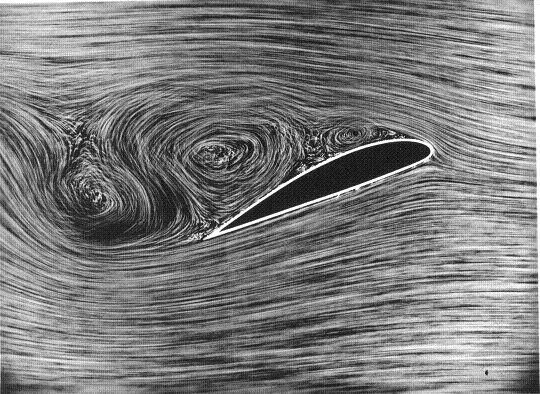
\includegraphics[width=0.3\textwidth]{stroemung1.PNG}
  }
  \subfigure{
    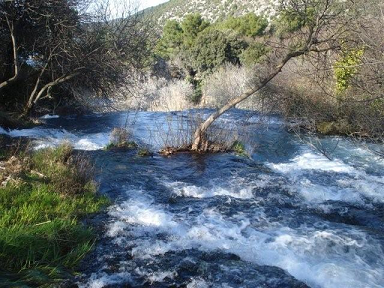
\includegraphics[width=0.3\textwidth]{stroemung2.PNG} 
  }
  \subfigure{
    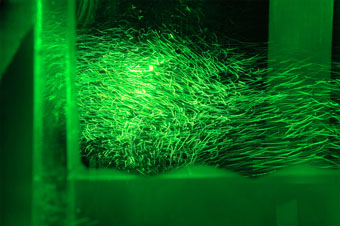
\includegraphics[width=0.3\textwidth]{stroemung3.PNG}
  }
  
  \caption{Bildunterschrift}
  \label{fig:xxxyyyzzzccc}
\end{figure}

\end{landscape}